\documentclass[a4]{beamer}
\usepackage{amssymb}
\usepackage{graphicx}
\usepackage{subfigure}
\usepackage{newlfont}
\usepackage{amsmath,amsthm,amsfonts}
%\usepackage{beamerthemesplit}
\usepackage{pgf,pgfarrows,pgfnodes,pgfautomata,pgfheaps,pgfshade}
\usepackage{mathptmx}  % Font Family
\usepackage{helvet}   % Font Family
\usepackage{color}

\mode<presentation> {
 \usetheme{Frankfurt} % was 
 \useinnertheme{rounded}
 \useoutertheme{infolines}
 \usefonttheme{serif}
 %\usecolortheme{wolverine}
% \usecolortheme{rose}
\usefonttheme{structurebold}
}

\setbeamercovered{dynamic}

\title[MA4413]{Statistics for Computing \\ {\normalsize MA4413 Lecture 3A}}
\author[Kevin O'Brien]{Kevin O'Brien \\ {\scriptsize Kevin.obrien@ul.ie}}
\date{Autumn Semester 2013}
\institute[Maths \& Stats]{Dept. of Mathematics \& Statistics, \\ University \textit{of} Limerick}

\renewcommand{\arraystretch}{1.5}

\begin{document}

\begin{frame}
\titlepage
\end{frame}

%--------------------------------------------------------------------------------------%
\frame{
\frametitle{Discrete Probability Distributions}

\begin{itemize}

\item Over the next set of lectures, we are now going to look at two important discrete probability distributions

\item The first is the \textbf{\emph{binomial}} probability distribution.

\item The second is the Poisson probability distribution.

\item In \texttt{R}, calculations are performed using the \texttt{binom} family of functions and \texttt{pois} family of functions respectively.
\end{itemize}

}


%--------------------------------------------------------------------------------------%
\frame{
\frametitle{Binomial Experiment}
A binomial experiment (also known as a Bernoulli trial) is a statistical experiment that has the following properties:
\begin{itemize}
\item The experiment consists of $n$ repeated trials.
\item Each trial can result in just two possible outcomes. We call one of these outcomes a \textbf{\emph{success}} and the other, a \textbf{\emph{failure}}.
\item The probability of success, denoted by $p$, is the same on every trial.
\item The trials are independent; that is, the outcome on one trial does not affect the outcome on other trials.
\end{itemize}
}
%--------------------------------------------------------------------------------------%
\frame{
\frametitle{Binomial Experiment}
Consider the following statistical experiment. You flip a coin five times and count the number of times the coin lands on heads. This is a binomial experiment because:
\begin{itemize}
\item The experiment consists of repeated trials. We flip a coin five times.
\item Each trial can result in just two possible outcomes : heads or tails.
\item The probability of success is constant : 0.5 on every trial.
\item The trials are independent; that is, getting heads on one trial does not affect whether we get heads on other trials.
\end{itemize}
}
%--------------------------------------------------------------------------------------%
\frame{
\frametitle{Binomial Probability}
\begin{itemize}
\item A binomial experiment with n trials and
probability $p$ of success will be denoted by
\[B(n, p)\]
\item Frequently, we are interested in the \textbf{\emph{number of successes}} in a binomial experiment, not in the order in which they occur.
\item Furthermore, we are interested in the probability of that number of successes.
\end{itemize}

}
%--------------------------------------------------------------------------------------%
\frame{
\frametitle{Binomial Probability}
The probability of exactly k successes in a binomial experiment B(n, p) is given by
\[ P(X=k) = P(k \mbox{ successes }) = \;^nC_k  \times p^{k} \times (1-p)^{n-k}\]

\begin{itemize}
\item X: Discrete random variable for the number of successes (variable name)
\item $k$ : Number of successes (numeric value)
\begin{itemize}
\item  $P(X=k)$ ``probability that the number of success is $k$".
\end{itemize}
\item $n$ : number of independent trials
\item $p$ : probability of a success in any of the $n$ trial.
\item $1-p$ : probability of a failure in any of the $n$ trial.
\end{itemize}

}


%--------------------------------------------------------------------------------------%
\frame{
\frametitle{Binomial Example }

Suppose a die is tossed 5 times. What is the probability of getting exactly 2 fours?

\textbf{Solution:}

This is a binomial experiment in which \begin{itemize}\item a success is defined as an outcome of `4'. \item the number of trials is equal to $n=5$, \item the number of successes is equal to $k=2$,\item the number of failures is equal to 3, \item  the probability of success on a single trial is 1/6, \item  the probability of failure on a single trial is 5/6.\end{itemize}
}
%--------------------------------------------------------------------------------------%
\begin{frame}[fragile]
\frametitle{Binomial Example }

Therefore, the probability of getting exactly 2 fours is:

\[P(X=2) = ^5C_2 \times (1/6)^2 \times (5/6)^3 = 0.161\]

Remark: $^5C_2 = 10$\\
\bigskip


\end{frame}

%--------------------------------------------------------%

\frame{
\frametitle{Binomial Example}

\begin{center}
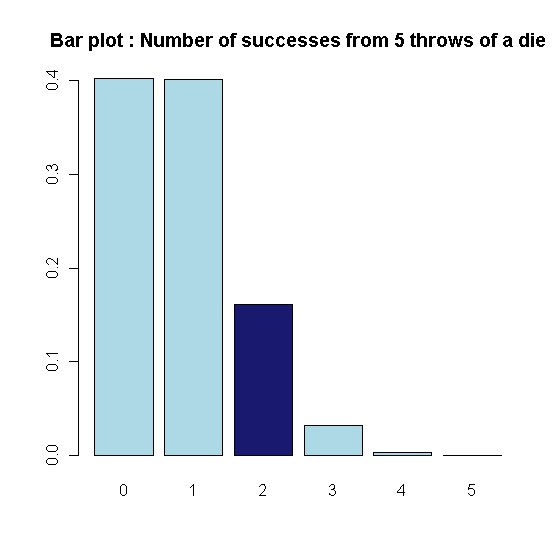
\includegraphics[scale=0.40]{3Bbarplot4}
\end{center}
}
%--------------------------------------------------------------------------------------%
\frame{
\frametitle{Binomial Probability}

\textbf{Remark} : The sum of the probabilities of each of the possible outcomes (i.e. no fours, one four etc) is equal to one.
\[P(X=0) + P(X = 1) + \ldots + P(X=5) = 1 \]

}
%--------------------------------------------------------%

\frame{
\frametitle{Binomial Example: At least two successes}

\begin{center}
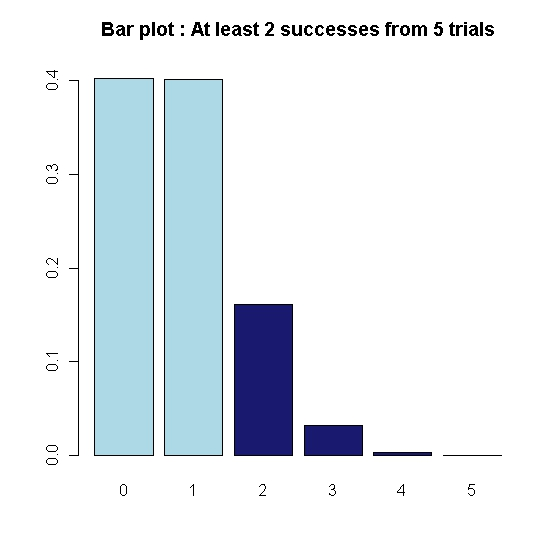
\includegraphics[scale=0.40]{3Bbarplot5}
\end{center}
}

%--------------------------------------------------------%

\frame{
\frametitle{Binomial Example: At least two successes}
\begin{itemize}
\item Suppose we were asked to find the probability of \textbf{\emph{at least}} 2 fours.
\item Can you suggest the most efficient way of computing this?
\item Suggestion: Compute $P(X=0)$ and $P(X = 1)$.
\item Together these probabilities are the complement probability of what we require.
\item $P(X \geq 2) = 1 - ( P(X=0) + P(X = 1))$.
\item (We will continue with this in future classes).
\end{itemize}
}
%--------------------------------------------------------------------------------------%
\frame{
\frametitle{Cumulative Distribution Function}


The cumulative distribution function (c.d.f.) of a discrete random variable $X$ is the function $F(t)$ which tells you the probability that X is less than or equal to t. \\ So if X has p.d.f. P(X = x), we have:

\[ F(t) = P(X \leq t) = \sum_{(i=0)}^{(i=t)} P(X = x) \]

In other words, for each value that X can be which is less than or equal to $t$, work out the probability that X is that value and add up all such results.

}




%--------------------------------------------------------%

\begin{frame}[fragile]
\frametitle{Binomial Example: Sample Problem}

Suppose there are twelve multiple choice questions in an English class quiz. Each question has five possible answers, and only one of them is correct. Find the probability of having four or less correct answers if a student attempts to answer every question at random.\\
\bigskip
\textbf{Solution:}
Since only one out of five possible answers is correct, the probability of answering a question correctly by random is $1/5=0.2$. We can find the probability of having exactly 4 correct answers by random attempts as follows.(Blackboard. Correct Answer is 13.29\%)
\begin{verbatim}
> dbinom(4, size=12, prob=0.2)
[1] 0.1329
\end{verbatim}
\end{frame}
%--------------------------------------------------------%

\frame{
\begin{itemize}
\item Binomial Coefficients / The Choose Operator
\item Definition: The Probability Mass Functions (pmf)
\item Binomial Distribution : Example
\end{itemize}
}
\frame{
\frametitle{Binomial Coefficients}

In the last class, we came across binomial coefficients. Informally, binomial coefficients are the number of ways $k$ items can be selected from a group of $n$ items. 
The binomial coefficient indexed by n and k is usually written as $^nC_k$ or
\[ {n \choose k}\].
$C$ is colloqially known as the ``choose operator".

\[ {n \choose k} = \frac{n!}{k! \times (n-k)!} \]

(We call the operator the choose operator. We will use both notations interchangeably.)
 

}
\frame{
\frametitle{Binomial Coefficients}

\begin{itemize}
\item $n!$ and $k!$ are the coefficients of $n$ and $k$ respectively.
\item $n! = n \times (n-1) \times (n-2) \times \ldots \times 2 \times 1$
\item For example $5! = 5\times4\times3\times2\times1 = 120$
\item $n! = n \times (n-1)!$
\item Importantly $0! = 1$ not 0.
\end{itemize}
\[ {6 \choose 2} = \frac{6!}{2! \times (6-2)!} = \frac{6!}{2! \times 4!}  \]\[\mbox{   } = \frac{6 \times 5 \times 4!}{2! \times 4!} 
 = 30/2 =15 \]
More examples of Binomial coefficients on blackboard.
}
%---------------------------------------------------------------------------%
\frame{
\frametitle{Probability Mass Function}
(Formally defining something mentioned previously)
\begin{itemize} \item a probability mass function (pmf) is a \textbf{\emph{function}}
that gives the probability that a discrete random variable is exactly equal to some
value.
\[P(X=k)\]
\item The probability mass function is often the primary means of defining a discrete
probability distribution
\item It is conventional to present the probability mass function in the form of a table.
\item The p.m.f of a value $k$ is often denoted $f(k)$.
\end{itemize}
}
%--------------------------------------------------------------------------------------%
\frame{
\frametitle{ Binomial Example 1 }
(Revision from Last Class)\\
Suppose a die is tossed 5 times. What is the probability of getting exactly 2 fours?

\textbf{Solution:} This is a binomial experiment in which the number of trials is equal to 5, the number of successes is equal to 2, and the probability of success on a single trial is 1/6 or about 0.167. 
\\
\bigskip
Therefore, the binomial probability is:

\[P(X=2) = ^5C_2 \times (1/6)^2 \times (5/6)^3 = 0.161\]
}

%--------------------------------------------------------------------------------------%
\frame{
\frametitle{ Binomial Example 2 }
Suppose there is a container that contains 6 items.  The probability that any one of these items is defective is 0.3. Suppose all six items are inspected. 
\begin{itemize}
\item What is the probability of 3 defective components?
\item What is the probability of 4 defective components?
\end{itemize}

\[ P(3\text{ defects}) = f(3) = P(X = 3) = {6\choose 3}0.3^3 (1-0.3)^{6-3} = 0.1852 \]
\[ P(4\text{ defects}) = f(4) = P(X = 4) = {6\choose 4}0.3^4 (1-0.3)^{6-4} = 0.0595 \]
}

%--------------------------------------------------------------------------------------%
\frame{
\frametitle{Probability Tables}
In the \textbf{Sulis} workspace there are two important tables used for this part of the course.


This class will feature a demonstration on how to read those tables.
\begin{itemize}
\item The Cumulative Binomial Tables (Murdoch Barnes Tables 1)
\item The Cumulative Poisson Tables (Murdoch Barnes Tables 2)
\end{itemize}

Please get a copy of each as soon as possible.

}

%---------------------------------------------------------------------------%
\frame{
\frametitle{Probability Tables}
\begin{itemize}
\item For some value $r$ the tables record the probability of $P(X \geq r)$.
\item The Student is required to locate the appropriate column based on the parameter values for the distribution in question.
\item A copy of the Murdoch Barnes Tables will be furnished to the student in the End of Year Exam. The Tables are not required for the first mid-term exam.
\item Knowledge of the sample space, partitioning of the sample points, and the complement rule are advised.
\end{itemize}
}
%---------------------------------------------------------------------------%


\frame{
\frametitle{Binomial Distribution : Using Tables}
It is estimated by a particular bank that 25\% of credit card customers pay only the minimum amount due on their monthly credit card bill and do not pay the total amount due. 50 credit card customers are randomly selected.
\begin{enumerate}
\item (3 marks)	What is the probability that 9 or more of the selected customers pay only the minimum amount due?
\item (3 marks) What is the probability that less than 6 of the selected customers pay only the minimum amount due?
\item (3 marks)	What is the probability that more than 5 but less than 10 of the selected customers pay only the minimum amount due?
\end{enumerate}

}

\frame{
\frametitle{Binomial Distribution : Using Tables}
Demonstration on Blackboard re: how to use tables in class.
\begin{enumerate}
\item $P(X \geq 9) = 0.9084$
\item $P(X < 6) = 1- P(X \geq 6) =1 - 0.9930 = 0.0070$
\item $P(6 \leq X \leq 9) = P(X \geq 6) - P(X \geq 10) = 0.9930 - 0.8363 = 0.1567$
\end{enumerate}

}


%------------------------------------------------------------------%
\frame{
\frametitle{Binomial Distribution: Expected Value and Variance}


If the random variable X has a binomial distribution with parameters n
and p, we write
\[ X \sim B(n,p) \]

Expectation and Variance
If $X \sim B(n,p)$, then:

\begin{itemize}
\item Expected Value of X : $E(X) = np$
\item Variance of X : $Var(X) = np(1-p)$
\end{itemize}

Suppose n=3 and p=0.5 
Then $E(X) = 1.5$ and $V(X) = 0.75$.

Remark: Referring to the expected value and variance may be used to validate
the assumption of a binomial distribution.

}
%---------------------------------------------------------------------------%
%------------------------------------------------------------------%
\frame{
\frametitle{Binomial Expected Value and Variance}


If the random variable X has a binomial distribution with parameters n
and p, we write
\[ X \sim B(n,p) \]

Expectation and Variance
If $X \sim B(n,p)$, then:

\begin{itemize}
\item Expected Value of X : E(X) = np
\item Variance of X : Var(X) = np(1-p)
\end{itemize}
}
%---------------------------------------------------------------------%
\begin{frame}
\frametitle{Binomial Distribution: Example 1}
\begin{itemize} \item Diagrams of the probability mass functions of the two binomial
distributions $B(10, 0.5)$ and $B(10, 0.25)$ are shown in the bar-plots (next slide). \item Which
is which? Give a reason for your answer.
\end{itemize}
\end{frame}
%---------------------------------------------------------------------%
\begin{frame}
\frametitle{Binomial Distribution}
\begin{figure}
  % Requires \usepackage{graphicx}
  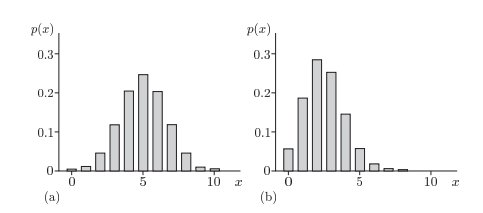
\includegraphics[scale=0.60]{4ABarCharts.jpg}\\
  \caption{Bar Charts}
\end{figure}
\end{frame}
%---------------------------------------------------------------------%
\begin{frame}
\frametitle{Binomial Distribution: Example 1}
\begin{itemize}
\item Clearly. Figure A is $B(10, 0.5)$ and Figure B is $B(10, 0.25)$.
\item The mean of B(10, 0.5) is 5, and the mean of B(10, 0.25) is 2.5. These values correspond to the apex of both distributions on the previous slide.
\item Also the variance of a binomial distribution corresponding to $B(10, 0.25)$ is $1.875$, while for $B(10, 0.25)$ it is $2.500$.
\item A visual inspection of the two bar-charts would indicate that Figure A has the higher variance.
\end{itemize}
\end{frame}
%---------------------------------------------------------------------%
\begin{frame}
\frametitle{Binomial Distribution: Example 2}
\textbf{Example}
\begin{itemize}
\item Components are placed into containers containing 100 items.
\item After an inspection of a large number of containers the average number of defective items was found to be 10 with a standard deviation of three.
\item Is the binomial distribution a good useful distribution, given the observed data?
\end{itemize}
\end{frame}
%---------------------------------------------------------------------%
\begin{frame}
\frametitle{Binomial Distribution: Example 2}

\begin{itemize}
\item Let the number of containers be the number of independent trials is $n=100$.
\item A success may be defined as a defective component.
\item The probability of a success is approximate $p=0.10$. (The probability of ``failure" is $1-p=0.9$).
\item The expected number of defective components is $np=10$, which concurs with our observed data.
\item The variance is computed as \[np(1-p) = 100 \times 0.1 \times 0.9 = 9\]
\item The observed standard deviation is 3 units, i.e. a variance of 9 square units.
\item Yes the binomial distribution is useful in this case.
\end{itemize}
\end{frame}
%------------------------------------------------------------------%
\frame{
\frametitle{Poisson Expected Value and Variance}


If the random variable X has a Poisson distribution with parameter $m$, we write
\[ X \sim Poisson(m) \]


\begin{itemize}
\item Expected Value of X : E(X) = m
\item Variance of X : $\mbox{Var}(X) = m$
\item Standard Deviation of X : $SD(X) = \sqrt{m}$
\end{itemize}
}
\end{document}


















\frame{
\frametitle{The Binomial Probability Distribution}
\begin{itemize}
\item The number of independent trials is denoted $n$.
\item The probability of a `success' is $p$
\item The expected number of `successes' from $n$ trials is $E(X) = np$
\end{itemize}
}

%---------------------------------------------------------------------------%
\frame{
\frametitle{Continuous Random Variables}

\begin{itemize}
\item Probability Density Function
\item Cumulative Density Function
\end{itemize}


If X is a continuous random variable then we can say that the probability of obtaining a \textbf{precise} value $x$ is infinitely small, i.e. close to zero.

\[P(X=x) \approx 0 \]

Consequently, for continuous random variables (only),  $P(X \leq x)$ and $P(X < x)$ can be used interchangeably.

\[P(X \leq x) \approx P(X < x) \]


}

%---------------------------------------------------------------------------%
\frame{
\frametitle{Continuous Uniform Distribution}
A random variable X is called a continuous uniform random variable over the interval $(a,b)$ if it's probability density function is given by

\[ f_{X}(x)  =  { 1 \over b-a}   \hspace{2cm}  \mbox{ when } a \leq x \leq b\]

The corresponding cumulative density function is

\[ F_x(x) = { x-a \over b-a}   \hspace{2cm}  \mbox{ when } a \leq x \leq b\]

}

%-----------------------------------------------------------------------------%

\frame{

The mean of the continuous uniform distribution is

\[ E(X) = {a+b \over 2}\]

\[ V(X) = {(b-a)^2\over12}\]
}

%-----------------------------------------------------------------------------%

\frame{
\frametitle{The Memoryless property}
The most interesting property of the exponential distribution is the \textbf{\emph{memoryless}} property. By this , we mean that if  the lifetime of a component is exponentially distributed, then an item which has been in use for some time is a good as a brand new item with regards to the likelihood of failure.

The exponential distribution is the only distribution that has this property.
}

%--------------------------------------------------------%

\frame{
\frametitle{Random Variables}
A pair of dice is thrown. Let X denote the minimum of the two numbers which occur.
Find the distributions and expected value of X.
}
%-------------------------------------------------------------%
\frame{
\frametitle{Random Variables}
A fair coin is tossed four times.
Let X denote the longest string of heads.
Find the distribution and expectation of X.}
%-------------------------------------------------------------%
\frame{\frametitle{Random Variables}
A fair coin is tossed until a head or five tails occurs.
Find the expected number E of tosses of the coin.}
%-------------------------------------------------------------%
\frame{\frametitle{Random Variables}A coin is weighted so that P(H) = 0.75 and P(T ) = 0.25

The coin is tossed three times. Let X denote the number of
heads that appear.
\begin{itemize}
\item (a) Find the distribution f of X.
\item (b) Find the expectation E(X).
\end{itemize}
}

%-------------------------------------------------------------%
\frame{
\begin{itemize}
\item Now consider an experiment with only two outcomes. Independent repeated trials of such an experiment are
called Bernoulli trials, named after the Swiss mathematician Jacob Bernoulli (1654\961705). \item The term \textbf{\emph{independent
trials}} means that the outcome of any trial does not depend on the previous outcomes (such as tossing a coin).
\item We will call one of the outcomes the ``success" and the other outcome the ``failure".
\end{itemize}
}

%-------------------------------------------------------------%
\frame{
\begin{itemize}
 \item
Let $p$ denote the probability of success in a Bernoulli trial, and so $q = 1 - p$ is the probability of failure.
A binomial experiment consists of a fixed number of Bernoulli trials. \item A binomial experiment with $n$ trials and
probability $p$ of success will be denoted by
\[B(n, p)\]
\end{itemize}
}
%-------------------------------------------------------------%

%---------------------------------------------------------------------------%
\frame{
\frametitle{Probability Mass Function}
\begin{itemize} \item a probability mass function (pmf) is a function that gives the probability that a discrete random variable is exactly equal to some value. \item The probability mass function is often the primary means of defining a discrete probability distribution \end{itemize}
}
%------------------------------------------------------------------%
\frame{
Thirty-eight students took the test. The X-axis shows various intervals of scores (the interval labeled 35 includes any score from 32.5 to 37.5). The Y-axis shows the number of students scoring in the interval or below the interval.

\textbf{\emph{cumulative frequency distribution}}A  can show either the actual frequencies at or below each interval (as shown here) or the percentage of the scores at or below each interval. The plot can be a histogram as shown here or a polygon.
}




\end{document}



%---------------------------------------------------------------------------------------------------------------%
%----R Code ----
%---------------------------------------------------------------------------------------------------------------%
n=60000
Y=numeric(n)
for ( i in 1:n){

X=floor(runif(100,1,7))
Y[i]=sum(X)
}

Y
hist(Y,breaks=seq(300,400,by=10),main=c("Totals of 100 Die Throws"),cex.lab=1.4,font.lab=2,xlab=c("Total Score"))

hist(Y,breaks=seq(300,400,by=20),main=c("Totals of 100 Die Throws"),cex.lab=1.4,font.lab=2,xlab=c("Total Score"))



Z=seq(1:n)
Y/Z

plot(Y/Z,type="l",col="red",main=c("Die Rolls: Running Average"),font.lab=2,ylab="Average Value", xlab=
" Number of Throws")
abline(h=3.5,col="green")


#####################################################

plot(Z,Z.y,pch=16,col="red",ylim=c(2.5,5.5),main=c("Variance"),font.lab=2,ylab=" ", xlab="X: Green  Y: Blue  Z: Red" )

points(Y,Y.y,pch=16,col="blue" )
points(X,X.y,pch=16,col="green" )
points(c(1000,1000,1000),c(3,4,5),pch=18,cex=1.2)
lines(c(1000,1000),c(2.75,5.25),lty=3)



n=100000
Y=numeric(n)
for ( i in 1:n){

X=floor(runif(100,1,7))
Y[i]=mean(X)
}

Y
hist(Y,breaks=seq(270,430,by=2),main=c("Mean of 100 Die Throws (n= 100,000)"),cex.lab=1.4,font.lab=2,xlab=c("Mean of 100 throws")) 
